\documentclass{jcgt}
\usepackage{tikz}
\usepackage{amsmath}
\usepackage{pgfplots}
\definecolor{darkgreen}{RGB}{0,192,0}

\setciteauthor{Alan Wolfe}
\setcitetitle{GPU Efficient Texture Based Bezier Curve Evaluation}

% Mark submissions with the date of submission using the following line:
%\submitted{\today}

% Once an article is accepted accepted, switch to the following line and comment the preceding one. The editor will supply the argument values.
\accepted{2014-02-07}{2014-02-07}{2014-02-07}{Editor Name}{3}{1}{1}{1}{2014}
\seturl{http://jcgt.org/published/0003/01/01/}


%%%%%%%%%%%%%%%%%%%%%%%%%%%%%%%%%%%%%%%%%%%%%%%%%


\begin{document}

\usetikzlibrary{arrows.meta}
\tikzset{>={Latex[width=3mm,length=3mm]}}

\title{GPU Efficient Texture Based Bezier Curve Evaluation}

\author
       {Alan Wolfe\\Blizzard Entertainment}

\teaser{
  \begin{tikzpicture}[x=5in,y=1.7in]
    \node[anchor=south west,inner sep=0] at (0,0) {
\includegraphics[width=5in,height=1.7in]{Teaser.png}};
    % representative line for where the quadratic bezier curve lives in the bilinear sampled texture
    \draw[yellow,->,line width=0.5mm]    (0.41,0.25) -- (0.58,0.75);
    \draw (0.08,0.25) node[] {\Huge{A}};
    \draw (0.25,0.25) node[] {\Huge{B}};
    \draw (0.08,0.75) node[] {\Huge{B}};
    \draw (0.25,0.75) node[] {\Huge{C}};    
  \end{tikzpicture}
  \caption{\textit{Left:} 2x2 texture containing control points for a quadratic Bezier curve in each color channel. \textit{Middle:} The texture as viewed with bilinear sampling. \textit{Right:} The resulting quadratic Bezier curves when sampling along the yellow line (Alpha curve omitted).}
  \label{fig:teaser}
}

\maketitle
\thispagestyle{firstpagestyle}

\begin{abstract}
\small
Modern graphics techniques expose internal parameters to allow re-use and to help separate the technical implementation from artistic usage cases.  A popular choice is to expose parameters as customizable curves and to quantize the curves into textures.  Quantization leads to either lower quality results, or more texture memory being used to accommodate higher sampling frequencies.  The technique presented in this paper leverages the capabilities of GPU texture samplers to allow more efficient storage and evaluation of both integral and rational Bezier curves of any order, resulting in higher fidelity for similar costs.  Piecewise curves, B-Splines and NURBS are addressed, and there are also limited applications towards vector graphics.
\end{abstract}


%-------------------------------------------------------------------------
\section{Introduction}
\label{sec:introduction}
There are two basic ways for a shader program to have customized curve data.  One way is to evaluate the curve on the CPU at discrete intervals and put those points into a texture that can be used by the GPU.  The other way is to pass curve control point data from the CPU to the shader program as shader constants, allowing the shader program to evaluate the curve at a given time $t$.

Baking curve points into a texture means that the shader program doesn't need to know what type of curve it was that made the data, nor how many control points it had, but comes at the loss of quality since there are a finite number of curve points sampled, and the data between points is just a linear interpolation between the samples.  If higher quality is desired, you can increase the resolution of the texture to trade accuracy for texture memory.

Passing control point data to a shader program as shader constants allows you to get high quality curve calculations, but comes at the cost of the shader program being written specifically for the type of curve you want to use, and also takes more shader program instructions to calculate specific curve points.

\begin{figure}
  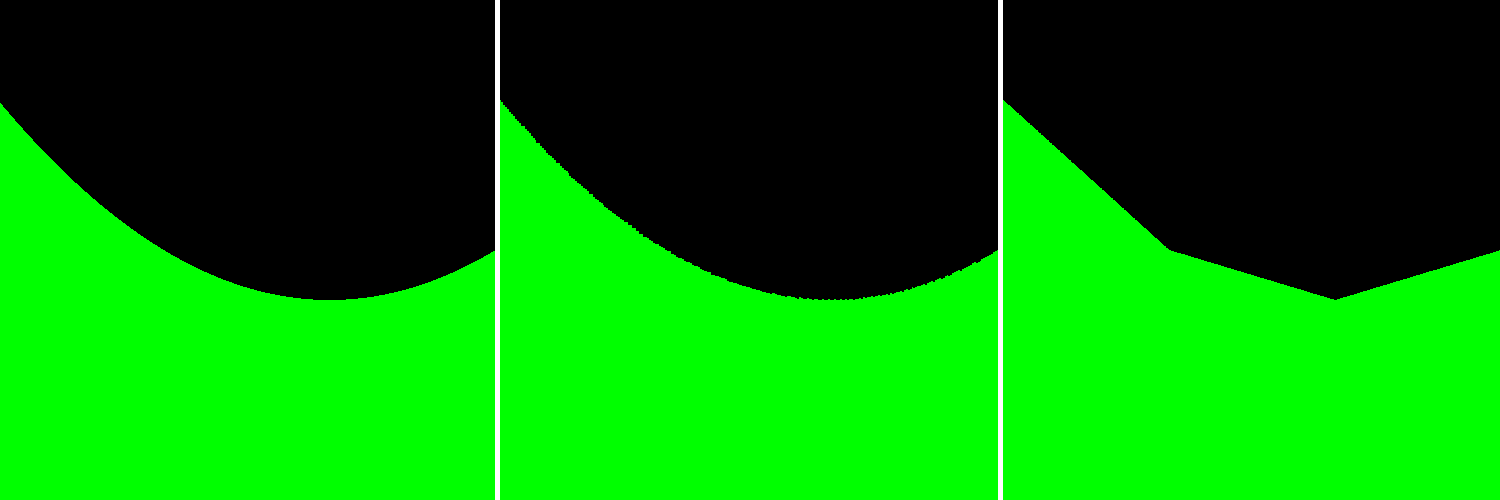
\includegraphics[width=5in]{Figure2.png}
  \caption{Quadratic Bezier curves (yellow) compared to a 4x1 baked out (quantized) texture for the same curve (red).  \textit{Left:} Curve evaluated from shader program constants. \textit{Right:}  The technique from this paper - the curve is stored in a 2x2 texture and a bilinear texture sample is taken to get each point on the curve.}
  \label{fig:quickcomparison}
\end{figure}

This paper shows a third method where:
\begin{itemize}
  \item The control points of the curves are encoded in a texture.
  \item The texture sampler calculates points on the curve before the data reaches the shader program.
  \item It gives accuracy results closer to that of shader constant curves, while having less calculation overhead.
  \item The technique can support both integral and rational Bezier curves of any order and can also be used for piecewise curves.
  \item The curve type must be decided on in advance, like when using the shader constant method.
  \item There are limited applications towards vector graphics.
\end{itemize}

A quick comparison of the visual quality of these three techniques can be seen in \autoref{fig:quickcomparison}.

Besides being useful for exposing internal parameters, the technique presented in this paper is also useful as an alternative to traditional shader look up tables, since this technique allows non linear interpolation between data points, where traditional lookup table textures only offer linear interpolation between data points.

%-------------------------------------------------------------------------
\section{The Technique}
\label{sec:thetechnique}

The core of this technique is that the $N$-dimensional linear texture interpolation capabilities on the GPU can be mathematically equivalent to De Casteljeau's algorithm for evaluating Bezier curves.  We can use linear texture sampling on textures of increasing dimensionalities to have the texture sampler calculate points on curves of increasing order.

\subsection{Intuition}

TODO: clean up the notation here!

One dimensional linear texture sampling is just the linear interpolation between two data points.  This is equivalent to the De Casteljeau algorithm when evaluating a linear curve of order 1.  In both cases, it is just linear interpolation between two values.

Two dimensional linear texture sampling (bilinear texture sampling) can be thought of as just the linear interpolation across the $y$ axis, of two linear interpolations across the $x$ axis (or an interpolation across the $x$ axis of two linear interpolations across the $y$ axis - order doesn't matter).  In other words, bilinear texture sampling is just the linear interpolation of two linear interpolations. 

The De Casteljeau algorithm for evaluating a quadratic curve (order 2) is also just a linear interpolation between two linear interpolations.  If the control points of the quadratic curve are $P_0,P_1,P_2$, let's call the first interpolation $\overline{P_0P_1}$ which is the interpolation between $P_0$ and $P_1$ for time $t$. The second linear interpolation is $\overline{P_1P_2}$ and is the interpolation between $P_1$ and $P_2$ for time $t$.  The final point on the curve will be the interpolation at time $t$ between $\overline{P_0P_1}$ and $\overline{P_1P_2}$, which we can call $\stackrel{\frown}{P_0P_1P_2}$.  

We could set up a texture such that the two $x$ axis interpolations would give us the values $\overline{P_0P_1}$ and $\overline{P_1P_2}$ respectively, and then the $y$ axis interpolation between those values would give us $\stackrel{\frown}{P_0P_1P_2}$.  When sampling, we would also use texture coordinates such it results in the same time $t$ value for interpolation on each axis.

To further see how bilinear interpolation can be equivalent to evaluating a quadratic Bezier curve with the De Casteljeau algorithm, \autoref{fig:decasteljeauBilinear} shows it visually, and you can also compare the GLSL source code in \autoref{lst:GLSLCurves}.

\begin{lstlisting}[caption={GLSL implementation of bilinear interpolation and the De Casteljeau algorithm for a quadratic Bezier curve.}, label={lst:GLSLCurves}]
float QuadraticBezier (
  in float t,
  in float P0, in float P1, in float P2
) {
    return mix(mix(P0,P1,t), mix(P1,P2,t), t);
}

// This function is equivelant to the function above when:
// u = t, v = t
// A = P0, B = P1, C = P1, D = P2
float BilinearInterpolate (
  in float u, in float v,
  in float A, in float B, in float C, in float D
) {
    return mix(mix(A,B,u), mix(C,D,u), v);
}

\end{lstlisting}


  \begin{figure}
    % bezier curve diagram
    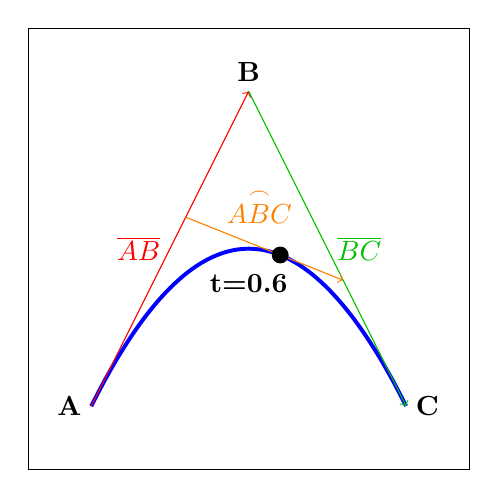
\begin{tikzpicture}[x=4cm,y=4cm]
      % border
      \draw (-0.2,-0.2) -- (1.2,-0.2) -- (1.2,1.2) -- (-0.2,1.2) -- (-0.2,-0.2);
      % 1d quadratic bezier curve with control points 0,1,0
      \draw[scale=1,domain=0:1,smooth,variable=\x,blue,line width=0.5mm] plot ({\x},{2*\x-2*\x*\x});    
      % control polygon / labels
      \draw[red,->]       (0.0,0.0) -- (0.5,1.0);
      \draw[darkgreen,->] (0.5,1.0) -- (1.0,0.0);
      \draw[red]          (0.25,0.5) node[anchor=east] {$\overline{AB}$};
      \draw[darkgreen]    (0.75,0.5) node[anchor=west] {$\overline{BC}$};
      % control point labels
      \draw (0.0,0.0) node[anchor=east]  {\bf{A}};
      \draw (0.5,1.0) node[anchor=south] {\bf{B}};
      \draw (1.0,0.0) node[anchor=west]  {\bf{C}};
      % draw a line from AB->AC for time = 0.75
      \draw[orange,->] (0.3,0.6) -- (0.8,0.4);
      \draw[orange] (0.40,0.55) node[anchor=south west] {$\stackrel{\frown}{ABC}$};
      % draw the point at t=0.6 and label underneath the curve
      \draw[black,fill=black] (0.6,0.48) circle (1mm);
      \draw[black] (0.5,0.45) node[anchor=north] {\bf{t}=0.6};
    \end{tikzpicture}
    % bilinear diagram
    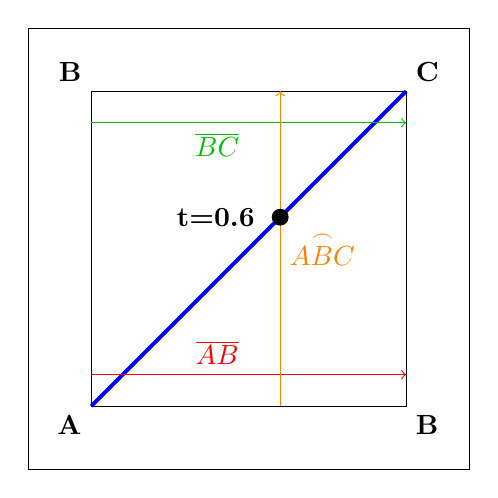
\begin{tikzpicture}[x=4cm,y=4cm]
        % border
        \draw (-0.2,-0.2) -- (1.2,-0.2) -- (1.2,1.2) -- (-0.2,1.2) -- (-0.2,-0.2);
        % box
        \draw (0,0) -- (1,0) -- (1,1) -- (0,1) -- (0,0);
        % representative line for where the quadratic bezier curve lives
        \draw[blue,line width=0.5mm] (0,0) -- (1,1);    
        % corner labels
        \draw (0,0) node[anchor=north east] {\bf{A}};
        \draw (1,0) node[anchor=north west] {\bf{B}};     
        \draw (0,1) node[anchor=south east] {\bf{B}};
        \draw (1,1) node[anchor=south west] {\bf{C}};     
        % x axis interpolation
        \draw[red,->]       (0.0,0.1) -- (1.0,0.1);
        \draw[red]          (0.4,0.1) node[anchor=south] {$\overline{AB}$};
        \draw[darkgreen,->] (0.0,0.9) -- (1.0,0.9);
        \draw[darkgreen]    (0.4,0.9) node[anchor=north] {$\overline{BC}$};
        % y axis interpolation
        \draw[orange,->]    (0.6,0.0) -- (0.6,1.0);
        \draw[orange]     (0.6,0.5) node[anchor=west] {$\stackrel{\frown}{ABC}$};
        % draw the point at t=0.6 and label for it
        \draw[black,fill=black] (0.6,0.6) circle (1mm);
        \draw[black] (0.55,0.6) node[anchor=east] {\bf{t}=0.6};
    \end{tikzpicture} 
    \caption{\textit{Left:} A quadratic Bezier curve evaluated at {\bf{t}}=0.6 for control points A,B,C using the De Casteljeau algorithm.  \textit{Right:} The De Casteljeau algorithm using bilinear interpolation.  Note that in this case, the X axis is evaluated before the Y, but the Y axis could be evaluated before the X for the same results.}
    \label{fig:decasteljeauBilinear}
  \end{figure}

The pattern continues for higher texture dimensions and curve orders as well.  Linear texture sampling of textures of dimension $N$ is just the linear interpolation between two linear texture samples of dimension $N-1$.  Using the De Casteljeau algorithm to evaluate a curve of order $N$ just means that you take a linear interpolation between curves of order $N-1$.

Compared to a quadratic curve evaluated with De Casteljeau's algorithm, bilinear texture sampling has two blend weights instead of one, and has four values to interpolate between instead of three, but you can set a texture up such that when you sample it a specific way, you get as output a quadratic Bezier curve.  Because of this, the De Casteljeau algorithm is a subset of the $N$-dimensional linear texture sampling available on the GPU.

It can be seen that the actual pixel value in a bilinear sampled texture is in the middle of a pixel.  That means that when calculating our texture coordinates for eg. a 2x2 texture, we must sample between pixel location $(0.5,0.5)$ and pixel location $(1.5,1.5)$ to get the correct results.

The common pixel formats contain four color channels –-- Red, Green, Blue and Alpha –-- which allows us to be able to evaluate four curves with a single texture read (\autoref{fig:texbilcurve}).

  \begin{figure}
    \begin{tikzpicture}[x=12.5cm,y=4.25cm]
      % border
      \draw (0cm,0cm) -- (12.5cm,0cm) -- (12.5cm,4.25cm) -- (0cm,4.25cm) -- (0cm, 0cm);   
      % raw texture, bilinear sampled texture, curve results
        \node[anchor=south west,inner sep=0] at (0.125cm,0.125cm) {
\includegraphics[width=4cm,height=4cm]{Figure4Texture.png}};
        \node[anchor=south west,inner sep=0] at (4.25cm,0.125cm) {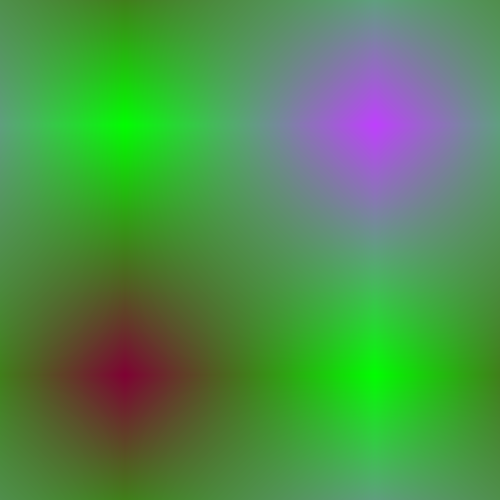
\includegraphics[width=4cm,height=4cm]{Figure4Bilinear.png}};
        \node[anchor=south west,inner sep=0] at (8.375cm,0.125cm) {
\includegraphics[width=4cm,height=4cm]{Figure4Curves.png}};
        % representative line for where the quadratic bezier curve lives
        \draw[yellow,->,line width=0.5mm]    (5.25cm,1.125cm) -- (7.25cm,3.125cm);    
        \draw (0.08,0.25) node[] {\Huge{A}};
        \draw (0.25,0.25) node[] {\Huge{B}};
        \draw (0.08,0.75) node[] {\Huge{B}};
        \draw (0.25,0.75) node[] {\Huge{C}};            
    \end{tikzpicture}
    \caption{\textit{Left:} a 2x2 texture storing control points for a quadratic Bezier curve in each color channel.  \textit{Middle:} The same texture as viewed when using bilinear texture sampling.  The yellow line indicates where texture samples are taken from to evaluate the quadratic Bezier curve. \textit{Right:} The curves resulting from sampling along the yellow line (Alpha curve omitted).}   
    \label{fig:texbilcurve}
  \end{figure}  

It is also possible to get points on curves of higher order by taking multiple texture reads and combining them either using the De Casteljeau algorithm, or by using the Bernstein form equation of Bezier curves.

\subsection{Mathematical Basis}

TODO: fix up notation to be consistant (Px vs A,B,C,D)

The De Casteljeau algorithm is equivalent to the Bernstein form of Bezier curves.

\begin{equation}
\bf{P(t)} = \sum\limits_{i=0}^n\binom {n} {i}(1-t)^{n-i}t^i\text{\bf{P}}_i
\label{eqn:bernsteinform}
\end{equation}

That they are equivalent means that the Bernstein form for a given $n$ must also be able to be evaluated by $n$-Linear interpolation.  A linear curve should be able to be evaluated by linear interpolation, a quadratic curve should be able to be evaluated by bilinear interpolation, a cubic curve should be able to be evaluated by trilinear interpolation, and so on.

When $n$ is $1$, to make a linear Bezier curve, the equation we get out is in fact just linear interpolation, so we can see that it's true in that case.

\begin{equation}
\bf{P(t)} = P_0(1-t) + P_1t
\label{eqn:bernsteinformn1}
\end{equation}

When $n$ is $2$, to make a quadratic Bezier curve with bilinear interpolation, the relationship is not as obvious.

\begin{equation}
\bf{P(t)} = P_0(1-t)^2 + P_12(1-t)t + P_2t^2
\label{eqn:bernsteinformn2}
\end{equation}

To see how that equation can be the same as bilinear interpolation, let's start with the equation for bilinear interpolation, which is just a linear interpolation between two other linear interpolations.  We'll use $t$ and $u$ as the interpolation weights of each interpolation.  We will linearly interpolate between linear interpolations $E(u)$ and $F(u)$ by $t$ to get out a result of $P(t,u)$

\begin{equation}
\begin{split}
\bf{E(u)} = P_0*(1-u) + P_1*u \\
\bf{F(u)} = P_2*(1-u) + P_3*u \\
\bf{P(t,u)} = E(u)*(1-t) + F(u)*t \\
\bf{P(t,u)} = (P_0*(1-u) + P_1*u)*(1-t) + (P_2*(1-u) + P_3*u)*t
\end{split}
\label{eqn:bilinearinterpolation}
\end{equation}

In our usage case of bilinear interpolation to evaluate Bernstein polynomials, $P_0$ will be $A$, $P_1$ and $P_2$ will both be $B$, and $P_3$ will be $C$.  Also, we set $t$ and $u$ equal in our usage case so we'll replace $u$ with $t$.  We will also replace $(1-t)$ with $s$ for readability.

\begin{equation}
\begin{split}
\bf{P(t)} = (A*s+B*t)*s + (B*s+C*t)*t \\
\bf{P(t)} = A*s^2+B*st + B*st+C*t^2 \\
\bf{P(t)} = A*s^2+B*2st+C*t^2
\end{split}
\label{eqn:bilinearinterpolation2}
\end{equation}

If we replace $A$,$B$,$C$ with $P_0$, $P_1$, $P_2$, and $s$ with $(1-t)$ we then get the familiar equation below, which is the Bernstein form of a quadratic Bezier curve.

\begin{equation}
\bf{P(t)} = P_0(1-t)^2+P_12(1-t)t+P_2t^2
\label{eqn:bilinearinterpolation3}
\end{equation}

This pattern continues for trilinear interpolation mapping to a cubic curve, and beyond.  $N$ dimensional linear texture sampling is just the linear interpolation between two linear texture samples of dimension $N-1$.  Bezier curves of order $N$ are just the linear interpolation between two bezier curves of order $N-1$.

\subsection{Accuracy}

  \begin{figure}
    \begin{tikzpicture}[x=12cm,y=4cm]
      % border
      \draw (0cm,0cm) rectangle (12cm,4cm);
      % raw texture, bilinear sampled texture, curve results
        \node[anchor=south west,inner sep=0] at (0cm,0cm) {
\includegraphics[width=4cm,height=4cm]{HighQuality.png}};
        \node[anchor=south west,inner sep=0] at (4cm,0cm) {
\includegraphics[width=4cm,height=4cm]{HighQualityZoom.png}};
        \node[anchor=south west,inner sep=0] at (8cm,0cm) {
\includegraphics[width=4cm,height=4cm]{LowQualityZoom.png}};
        % representative line for where the quadratic bezier curve lives
        \draw[yellow] (0.11,0.35) rectangle (0.21,0.65);    
          
    \end{tikzpicture}
    \caption{\textit{Left:} Sampled curves.  \textit{Middle:} Zooming in on a curve calculated with shader program constants.  \textit{Right:} Zooming in on a curve calculated using the method in this paper}   
    \label{fig:quickaccuracy}
  \end{figure}  

A limitation with this technique is that control points can only take values that can be stored and recalled from the specific texture format being used, which puts a limitation on the range of values able to be used, as well as the precision of the values stored.

Furthermore, the fractional position of a texel used in the interpolation formulas is limited to 256 values due to it being calculated with a 9 bit (1.8) fixed point format \cite{NVIDIA}.

The accuracy issues can be seen in \autoref{fig:quickaccuracy}, although the accuracy can still be significantly higher than a baked out curve using the same number of pixels as seen in \autoref{fig:quickcomparison}.

%-------------------------------------------------------------------------
\section{Texture Dimensionality}
\label{sec:texturedimensionality}

While this technique is able to be used with any texture dimensionality, there are different characteristics for each choice.  Those characteristics will be explored here.

\newcommand*\circled[1]{\tikz[baseline=(char.base)]{
            \node[shape=circle,draw] (char) {#1};}}

\begin{figure}
  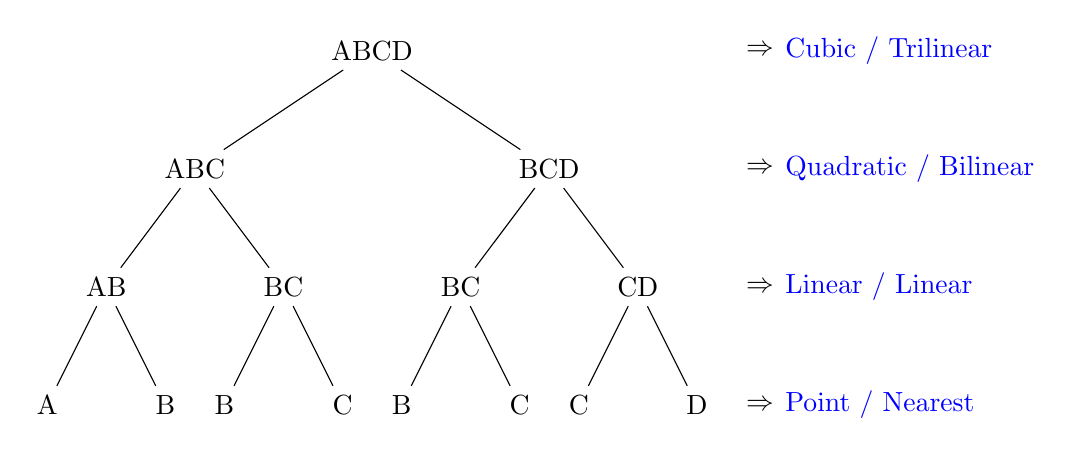
\begin{tikzpicture}[level/.style={sibling distance = 4.5cm/#1, level distance = 1.5cm}] 
    \begin{scope}[shift={(-6cm,0)}]
      \node (Root) {\circled{ABCD}}
          child{ node{\circled{ABC}}
                  child{ node {\circled{AB}}
                    child{ node {\circled{A}}}
                    child{ node {\circled{B}}}            
                  }
                  child{ node {\circled{BC}}
                    child{ node {\circled{B}}}
                    child{ node {\circled{C}}}            
                  }                            
          }
          child{ node {\circled{BCD}}
                  child{ node {\circled{BC}}
                    child{ node {\circled{B}}}
                    child{ node {\circled{C}}}
                  }  
                  child{ node {\circled{CD}}
                    child{ node {\circled{C}}}
                    child{ node {\circled{D}}}
                  }  
          }
      ; 

      % Comments for each level
      \begin{scope}[every node/.style={right}]
        \path (Root      -| Root-2-2-2) ++(5mm,0) node {$\Rightarrow$} ++(5mm,0) node [blue] {Cubic / Trilinear};
        \path (Root-1    -| Root-2-2-2) ++(5mm,0) node {$\Rightarrow$} ++(5mm,0) node [blue] {Quadratic / Bilinear};
        \path (Root-1-1  -| Root-2-2-2) ++(5mm,0) node {$\Rightarrow$} ++(5mm,0) node [blue] {Linear / Linear};
        \path (Root-1-1-1-| Root-2-2-2) ++(5mm,0) node {$\Rightarrow$} ++(5mm,0) node [blue] {Point / Nearest};
      \end{scope}
    \end{scope}   
  \end{tikzpicture}
  \caption{A tree showing the De Casteljeau algorithm for a cubic curve.  The labels on the right show what type of curves are evaluated at that level, as well as the $N$ dimensional sampling that is required to evaluate nodes at that level with a single texture read.}
  \label{fig:decdimensionality}
\end{figure}  

\subsection{One Dimensional Textures}

Using one dimensional textures, the built in texture interpolation is only able to perform linear interpolation, which allows calculations of only 1st order (linear) Bezier curves (\autoref{fig:decdimensionality}).

Since the De Casteljeau algorithm just interpolates between linear interpolations, we can take more texture samples and combine them in the shader program to get higher order curves.  For an order $N$ Bezier curve, the De Casteljeau algorithm requires $2^{N-1}$ linear interpolations for the linear level of the tree.  You need two pixels to perform a linear interpolation, so it seems that we would need $2^N$ pixels to store a curve of order $N$ in a 1 dimensional textures.  For a cubic curve, that would look like this: $[P_0,P_1,P_1,P_2,P_1,P_2,P_2,P_3]$.

We can do better than that though.  Firstly, there are redundant lerps in the list for lerping between $P_1$ and $P_2$.  As the order of the curve increases, the number of redundancies increase as well.  We don't want to have to pay the cost of pixel storage and texture samples for redundancies, so because we have $N+1$ control points and we only ever sample between  $P_i$ and $P_{i+1}$, we only need to store $N$ lerps in the 1 dimensional texture, which would mean we would need $N*2$ pixels.  A cubic curve would then look like this:  $[P_0,P_1,P_1,P_2,P_2,P_3]$.

After eliminating redundant lerps, we can see that there are redundant data values in our texture.  $P_1$ and $P_2$ each show up twice.  As the order of the curve increases, we would notice the pattern that all control points show up twice except the end points.  We can remove these redundancies and still be able to get the same information out.  The result of removing these redundancies is that our texture only needs to contain each control point once, which means we only need $N+1$ pixels to encode a curve of order $N$.  The cubic curve now looks like this: $[P_0,P_1,P_2,P_3]$. 

If $M$ piecewise curves are desired, we multiply the number of pixels used for one curve by $M$.  The size of the one dimensional texture needed for $M$ piecewise curves, each of degree $N$ is $M*(N+1)$. Two piecewise cubic curves encoded into a texture would be 8 pixels in size and look like this: $[P_0,P_1,P_2,P_3,P_4,P_5,P_6,P_7]$

It's often the case that you want $C0$ continuity for piecewise curves though, which in the example would give $P_4$ the same value as $P_3$.  If your piecewise curves always had $C0$ continuity, you could remove the redundant control point for every curve after the first, which would make it so the size of the texture required became $N*M+1$ (\autoref{fig:texlayeout1d}).

  \begin{figure}
    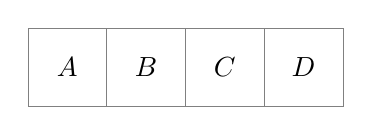
\begin{tikzpicture}
      \draw[step=1cm,gray,very thin] (0,0) grid (4,1);
      \draw (0.5,0.5) node {$A$};
      \draw (1.5,0.5) node {$B$};
      \draw (2.5,0.5) node {$C$};
      \draw (3.5,0.5) node {$D$};
    \end{tikzpicture}

    \vspace{5mm}

    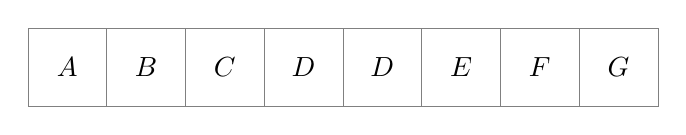
\begin{tikzpicture}
      \draw[step=1cm,gray,very thin] (0,0) grid (8,1);
      \draw (0.5,0.5) node {$A$};
      \draw (1.5,0.5) node {$B$};
      \draw (2.5,0.5) node {$C$};
      \draw (3.5,0.5) node {$D$};
      \draw (4.5,0.5) node {$D$};
      \draw (5.5,0.5) node {$E$};
      \draw (6.5,0.5) node {$F$};
      \draw (7.5,0.5) node {$G$};     
    \end{tikzpicture}   

    \vspace{5mm}

    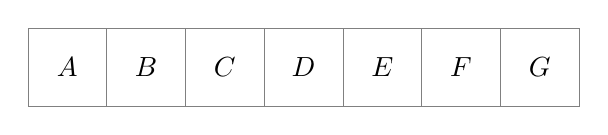
\begin{tikzpicture}
      \draw[step=1cm,gray,very thin] (0,0) grid (7,1);
      \draw (0.5,0.5) node {$A$};
      \draw (1.5,0.5) node {$B$};
      \draw (2.5,0.5) node {$C$};
      \draw (3.5,0.5) node {$D$};
      \draw (4.5,0.5) node {$E$};
      \draw (5.5,0.5) node {$F$};
      \draw (6.5,0.5) node {$G$};     
    \end{tikzpicture}      
    \caption{\textit{Top:} A cubic curve with control points $A,B,C,D$ encoded in a 1d texture with a size of 4 pixels.  \textit{Middle:} Two piecewise curves encoded in a 1d texture.  The control points for the first curve are $A,B,C,D$ and the control points for the second curve are $D,E,F,G$.  \textit{Bottom:} With $C0$ continuity, a redundant $D$ can be removed to store these curves in 7 pixels instead of 8. }    
    \label{fig:texlayeout1d}
  \end{figure}

Taking $N$ linearly interpolated texture samples from a one dimensional texture of size $N+1$ gives us the linear interpolated values we would need to continue to perform the De Casteljeau algorithm.  We can compute the final curve point either by doing that, or by plugging the values into the Bernstein form equation of Bezier curves.

In the case of a cubic curve with control points $A,B,C,D$, the one dimensional texture will be 4 pixels in size, and three texture reads will need to be done to get the interpolations for $\overline{AB},\overline{BC},\overline{CD}$.  Those will then need to be combined using either the De Casteljeau algorithm, or by using the Bernstein form of a quadratic Bezier curve ($P = A*s^2 + B*st + C*t^2$) to elevate those three points from order 1 to order 3, to get the final point $\stackrel{\frown}{ABCD}$.  Sample code of this example is provided in \autoref{lst:GLSLCubicTexture1D}.

\begin{lstlisting}[caption={GLSL for evaluating a cubic curve encoded in a 4 pixel 1d texture.  Linear texture sampling is used to evaluate the linear level of the De Casteljeau algorithm, then the process is continued both with the De Casteljeau algorithm, as well as the Bernstein form of a quadratic Bezier curve.}, label={lst:GLSLCubicTexture1D}]
// 4 pixel 1d texture with control points encoded: A,B,C,D
uniform sampler1D uSampler; 
const float c_textureSize = 4.0;

vec4 CubicCurveFromTexture1D_DeCasteljeau(in float t) {
    vec4 AB = texture(uSampler, (t + 0.5) / c_textureSize);
    vec4 BC = texture(uSampler, (t + 1.5) / c_textureSize;
    vec4 CD = texture(uSampler, (t + 2.5) / c_textureSize);
    vec4 ABC = mix(AB, BC, t);
    vec4 BCD = mix(BC, CD, t);
    return mix(ABC, BCD, t);
}

vec4 CubicCurveFromTexture1D_Bernstein(in float t) {
    vec4 AB = texture(uSampler, (t + 0.5) / c_textureSize);
    vec4 BC = texture(uSampler, (t + 1.5) / c_textureSize);
    vec4 CD = texture(uSampler, (t + 2.5) / c_textureSize);
    float s = (1 - t);
    float s2 = s * s;
    float t2 = t * t;
    // Quadratic Bezier Curve = A*s*s + B*2*s*t + C*t*t
    return AB*s2 + BC*2.0*s*t + CD*t2;
}
\end{lstlisting}

\subsection{Two Dimensional Textures}
Using two dimensional textures allows the texture interpolator to perform bilinear interpolation, which allows calculations of 2nd order (quadratic) Bezier curves (\autoref{fig:decdimensionality}).

This allows us to either calculate a quadratic Bezier curve with a single texture read, or allows us to get the quadratic level values needed to make a higher order curve.

Knowing that a quadratic curve is just the linear interpolation of time $t$ between the points on two linear curves at time $t$, we have to find a way to make a texture that will cause this to happen with bilinear interpolation.  The result is that if we have a $2$x$2$ texture, the top two pixels should be $P_0$ and $P_1$ and the bottom two pixels should be $P_1$ and $P_2$.  When we do a bilinear interpolation such that we plug $t$ into both $u$ and $v$, the end result will be that $\overline{P_0P_1}$ and $\overline{P_1P_2}$ will be calculated from the $u$ axis interpolation, and then those two will be linearly interpolated across the $v$ axis to give us the final result.

Knowing that we can linearly interpolate between two quadratic curves to create a cubic curve, and that we can combine three quadratic curves to create a quartic curve, the pattern seems to be that we need a texture size of $(2,2*(N-1))$ to encode a curve of order $N$ into a two dimensional texture.

When actually creating that texture, we would once again see redundancies however.  For a cubic curve with control points $P_0,P_1,P_2,P_3$ we would see that the top row of pixels was $P_0,P_1$, then the next row was $P_1,P_2$.  That would be our first quadratic curve.  The third row would start our second quadratic curve which would be $P_1,P_2$ and then the fourth and final row would be $P_2,P_3$.  In this case, $P_1,P_2$ is redundant.  If we increased the order of the curve, the pattern that we would see is that every curve after the first curve would have a redundant row.

Removing that redundant row, it means that we start with a $2$x$2$ texture for a quadratic curve, and then just add a row of pixels for each order above quadratic.  That makes the size of our texture required be only $(2,N)$.

If $M$ piecewise curves are desired, each of degree $N$, we can encode them across the $X$ axis to require a texture size of $(2*M,N)$ (\autoref{fig:texlayeout2d}).

  \begin{figure}
    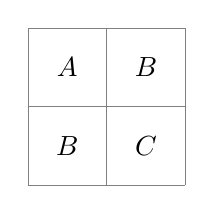
\begin{tikzpicture}
      \draw[step=1cm,gray,very thin] (0,0) grid (2,-2);
      \draw (0.5,-0.5) node {$A$};
      \draw (1.5,-0.5) node {$B$};
      \draw (0.5,-1.5) node {$B$};
      \draw (1.5,-1.5) node {$C$};     
    \end{tikzpicture}
    \hspace{5mm}  
    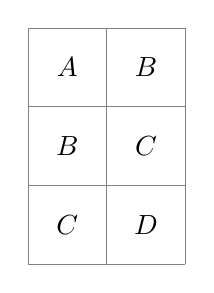
\begin{tikzpicture}
      \draw[step=1cm,gray,very thin] (0,0) grid (2,-3);
      \draw (0.5,-0.5) node {$A$};
      \draw (1.5,-0.5) node {$B$};
      \draw (0.5,-1.5) node {$B$};
      \draw (1.5,-1.5) node {$C$};
      \draw (0.5,-2.5) node {$C$};
      \draw (1.5,-2.5) node {$D$};      
    \end{tikzpicture}
    \hspace{5mm}
    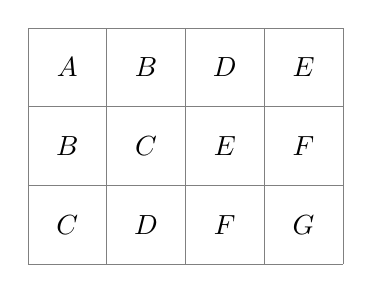
\begin{tikzpicture}
      \draw[step=1cm,gray,very thin] (0,0) grid (4,-3);
      \draw (0.5,-0.5) node {$A$};
      \draw (1.5,-0.5) node {$B$};
      \draw (0.5,-1.5) node {$B$};
      \draw (1.5,-1.5) node {$C$};
      \draw (0.5,-2.5) node {$C$};
      \draw (1.5,-2.5) node {$D$};  

      \draw (2.5,-0.5) node {$D$};
      \draw (3.5,-0.5) node {$E$};
      \draw (2.5,-1.5) node {$E$};
      \draw (3.5,-1.5) node {$F$};
      \draw (2.5,-2.5) node {$F$};
      \draw (3.5,-2.5) node {$G$};          
    \end{tikzpicture}
    \caption{\textit{Left:} A quadratic curve with control points $A,B,C$ encoded in a 2d texture that is $(2,2)$ in size. \textit{Middle:} A cubic curve with control points $A,B,C,D$ encoded in a 2d texture that is $(2,3)$ in size.  \textit{Right:} Two piecewise curves encoded in a 2d texture that is $(4,3)$ in size.  The control points for the first curve are $A,B,C,D$ and the control points for the second curve are $D,E,F,G$.} 
    \label{fig:texlayeout2d}
  \end{figure}  

GLSL source code is also provided below to help see how that would work for sampling a cubic curve from a two dimensional texture, with two bilinear texture samples combined to create the final cubic curve.

\begin{lstlisting}[caption={GLSL for evaluating a cubic curve encoded in a $(2,4)$ pixel 2d texture.  Bilinear texture sampling used to evaluate the first two levels of the De Casteljeau algorithm, then the process is continued both with the De Casteljeau algorithm, as well as the Bernstein form of a linear Bezier curve (lerp).}, label={lst:GLSLCubicTexture2D}]
// 2x4 2d texture, rounded to the nearest powers of 2 from 2x3.
uniform sampler2D uSampler; 
const vec2 c_textureSize = vec2(2.0,4.0);

vec4 CubicCurveFromTexture2D_DeCasteljeau(in float t) {
    vec4 ABC = texture(uSampler, (vec2(0.5, 0.5)+t) / c_textureSize);
    vec4 BCD = texture(uSampler, (vec2(0.5, 1.5)+t) / c_textureSize);
    return mix(ABC, BCD, t);
}

vec4 CubicCurveFromTexture2D_Bernstein(in float t) {
    vec4 ABC = texture(uSampler, (vec2(0.5, 0.5)+t) / c_textureSize);
    vec4 BCD = texture(uSampler, (vec2(0.5, 1.5)+t) / c_textureSize);
    float s = (1 - t);
    // Linear Bezier Curve = A*s + B*t
    return ABC*s + BCD*t;
}
\end{lstlisting}

\subsection{Three Dimensional Textures}

Using three dimensional textures (often referred to as volumetric textures) allows the texture interpolator to evaluate trilinear interpolation, which allows calculations of 3rd order (cubic) Bezier curves (\autoref{fig:decdimensionality}).

This allows us to either calculate a cubic Bezier curve with a single texture read, or allows us to get the cubic level values needed to make a higher order curve.

Knowing that a cubic curve is just the linear interpolation of time $t$ between the points on two quadratic curves at time $t$, we need to find a way to set up a 3d texture to make this happen with trilinear texture sampling.  With a $2$x$2$x$2$ texture, the front $2$x$2$ pixels would encode a quadratic curve for $P_0,P_1,P_2$ and the back $2$x$2$ pixels would encode a quadratic curve for $P_1,P_2,P_3$.  Then, when we sample the texture, plugging $t$ into $u,v$ and $w$, the result will be that it will calculate the points on the quadratic curves $P_0,P_1,P_2$ at time $t$ and also $P_1,P_2,P_3$ at time $t$, and then will interpolate across the $w$ axis to give us the final result.

You can combine two cubic curves to make a quartic curve, or three cubic curves to make a quintic curve.  If you were to put $2$x$2$x$2$ cubic curves back to back, you would notice a redundancy like we saw in lower dimensionality textures.  Instead of going that route though, we can just build on what we did for two dimensional textures.

The size of a three dimensional texture needed to encode a curve of degree $N$ is $(2,N-1,2)$.  If you wanted to store $M$ piecewise curves, each of degree $N$, the formula becomes $(2*M,N-1,2)$ (\autoref{fig:texlayeout3d}).

\begin{figure}
    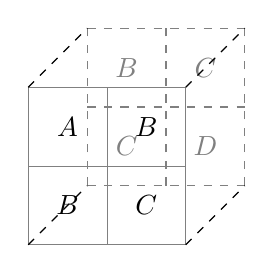
\begin{tikzpicture}
      \draw[step=1cm,gray,very thin] (0,0,0) grid (2,-2,0);
      \draw (0.5,-0.5) node {$A$};
      \draw (1.5,-0.5) node {$B$};
      \draw (0.5,-1.5) node {$B$};
      \draw (1.5,-1.5) node {$C$};

      \begin{scope}[shift={(0.75,0.75,0)}]
        \draw[step=1cm,gray,dashed] (0,0,0) grid (2,-2,0);
        \draw[gray] (0.5,-0.5) node {$B$};
        \draw[gray] (1.5,-0.5) node {$C$};
        \draw[gray] (0.5,-1.5) node {$C$};
        \draw[gray] (1.5,-1.5) node {$D$};
      \end{scope}

      \draw[dashed] (0,0,0) -- (0.75, 0.75,0);
      \draw[dashed] (2,0,0) -- (2.75, 0.75,0);
      \draw[dashed] (0,-2,0) -- (0.75,-1.25,0);
      \draw[dashed] (2,-2,0) -- (2.75,-1.25,0);
    \end{tikzpicture}
    \hspace{5mm}
    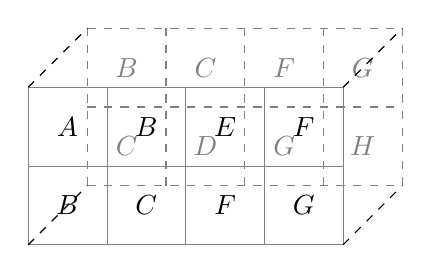
\begin{tikzpicture}
      \draw[step=1cm,gray,very thin] (0,0,0) grid (4,-2,0);
      \draw (0.5,-0.5) node {$A$};
      \draw (1.5,-0.5) node {$B$};
      \draw (0.5,-1.5) node {$B$};
      \draw (1.5,-1.5) node {$C$};

      \draw (2.5,-0.5) node {$E$};
      \draw (3.5,-0.5) node {$F$};
      \draw (2.5,-1.5) node {$F$};
      \draw (3.5,-1.5) node {$G$};

      \begin{scope}[shift={(0.75,0.75,0)}]
        \draw[step=1cm,gray,dashed] (0,0,0) grid (4,-2,0);
        \draw[gray] (0.5,-0.5) node {$B$};
        \draw[gray] (1.5,-0.5) node {$C$};
        \draw[gray] (0.5,-1.5) node {$C$};
        \draw[gray] (1.5,-1.5) node {$D$};

        \draw[gray] (2.5,-0.5) node {$F$};
        \draw[gray] (3.5,-0.5) node {$G$};
        \draw[gray] (2.5,-1.5) node {$G$};
        \draw[gray] (3.5,-1.5) node {$H$};
      \end{scope}

      \draw[dashed] (0,0,0) -- (0.75, 0.75,0);
      \draw[dashed] (4,0,0) -- (4.75, 0.75,0);
      \draw[dashed] (0,-2,0) -- (0.75,-1.25,0);
      \draw[dashed] (4,-2,0) -- (4.75,-1.25,0);
    \end{tikzpicture}

    \vspace{5mm}

    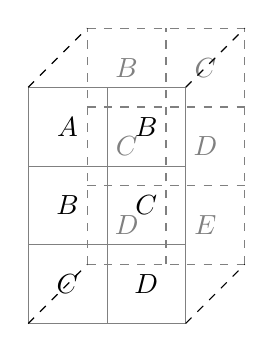
\begin{tikzpicture}
      \draw[step=1cm,gray,very thin] (0,0,0) grid (2,-3,0);
      \draw (0.5,-0.5) node {$A$};
      \draw (1.5,-0.5) node {$B$};
      \draw (0.5,-1.5) node {$B$};
      \draw (1.5,-1.5) node {$C$};
      \draw (0.5,-2.5) node {$C$};
      \draw (1.5,-2.5) node {$D$};

      \begin{scope}[shift={(0.75,0.75,0)}]
        \draw[step=1cm,gray,dashed] (0,0,0) grid (2,-3,0);
        \draw[gray] (0.5,-0.5) node {$B$};
        \draw[gray] (1.5,-0.5) node {$C$};
        \draw[gray] (0.5,-1.5) node {$C$};
        \draw[gray] (1.5,-1.5) node {$D$};
        \draw[gray] (0.5,-2.5) node {$D$};
        \draw[gray] (1.5,-2.5) node {$E$};
      \end{scope}

      \draw[dashed] (0,0,0) -- (0.75, 0.75,0);
      \draw[dashed] (2,0,0) -- (2.75, 0.75,0);
      \draw[dashed] (0,-3,0) -- (0.75,-2.25,0);
      \draw[dashed] (2,-3,0) -- (2.75,-2.25,0);
    \end{tikzpicture}
    \hspace{5mm}
    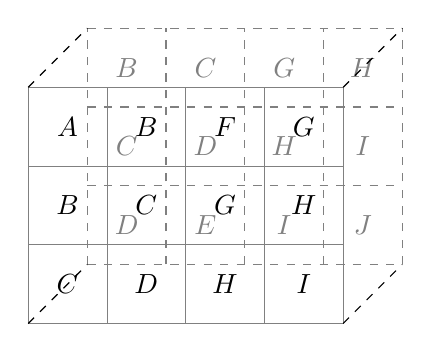
\begin{tikzpicture}
      \draw[step=1cm,gray,very thin] (0,0,0) grid (4,-3,0);
      \draw (0.5,-0.5) node {$A$};
      \draw (1.5,-0.5) node {$B$};
      \draw (0.5,-1.5) node {$B$};
      \draw (1.5,-1.5) node {$C$};
      \draw (0.5,-2.5) node {$C$};
      \draw (1.5,-2.5) node {$D$};

      \draw (2.5,-0.5) node {$F$};
      \draw (3.5,-0.5) node {$G$};
      \draw (2.5,-1.5) node {$G$};
      \draw (3.5,-1.5) node {$H$};
      \draw (2.5,-2.5) node {$H$};
      \draw (3.5,-2.5) node {$I$};

      \begin{scope}[shift={(0.75,0.75,0)}]
        \draw[step=1cm,gray,dashed] (0,0,0) grid (4,-3,0);
        \draw[gray] (0.5,-0.5) node {$B$};
        \draw[gray] (1.5,-0.5) node {$C$};
        \draw[gray] (0.5,-1.5) node {$C$};
        \draw[gray] (1.5,-1.5) node {$D$};
        \draw[gray] (0.5,-2.5) node {$D$};
        \draw[gray] (1.5,-2.5) node {$E$};


        \draw[gray] (2.5,-0.5) node {$G$};
        \draw[gray] (3.5,-0.5) node {$H$};
        \draw[gray] (2.5,-1.5) node {$H$};
        \draw[gray] (3.5,-1.5) node {$I$};
        \draw[gray] (2.5,-2.5) node {$I$};
        \draw[gray] (3.5,-2.5) node {$J$};
      \end{scope}

      \draw[dashed] (0,0,0) -- (0.75, 0.75,0);
      \draw[dashed] (4,0,0) -- (4.75, 0.75,0);
      \draw[dashed] (0,-3,0) -- (0.75,-2.25,0);
      \draw[dashed] (4,-3,0) -- (4.75,-2.25,0);
    \end{tikzpicture}

    \caption{\textit{Top Left:} A cubic curve encoded in a $(2,2,2)$ sized texture, decoded with a single trilinear texture sample. \textit{Top Right:}  Two piecewise cubic curves encoded in a $(4,2,2)$ sized texture, decoded with a single trilinear texture sample.  \textit{Bottom Left:} A Quartic curve encoded in a $(2,3,2)$ sized texture, decoded with two trilinear texture samples. \textit{Bottom Right:} Two piecewise quartic curves encoded in a $(4,3,2)$ sized texture, decoded with two trilinear texture samples.} 
    \label{fig:texlayeout3d}
  \end{figure}  

Below is some GLSL source code showing how you would sample a cubic curve stored in a 3d 2x2x2 texture, using trilinear texture sampling.

\begin{lstlisting}[caption={GLSL for evaluating a cubic curve encoded in a $(2,2,2)$ pixel 3d texture.  Trilinear texture sampling used to evaluate all three levels of the De Casteljeau algorithm.}, label={lst:GLSLCubicTexture3D}]
// 2x2x2 3d texture.
uniform sampler2D uSampler; 
const vec3 c_textureSize = vec3(2.0, 2.0, 2.0);

vec4 CubicCurveFromTexture3D(in float t) {
    return texture(uSampler, vec3(0.5 + t) / c_textureSize);
}
\end{lstlisting} 

\subsection{Summary of Texture Dimensionality}

Increasing texture dimensionality allows you to evaluate the same order curve with fewer texture reads but comes at the cost of using more texture memory.  We evaluated texture dimensions one, two and three, but the pattern continues for higher dimensions as well.

The table below is a comparison of texture dimensionality options.  $M$ is the number of piecewise curves being stored and $N$ is the order of the curve.  To get an idea of how dimensionality and order affects the size of the required textures, take a look at \autoref{fig:pixelcount}.

\begin{tabular}{|l|l|l|l|l|}
\hline
 & \bf{Min. Order} & \bf{\# Samples} & \bf{Dimensions} & \bf{\# Pixels} \\ \hline
\bf{1D} & 1 (Linear) & $N$ & $(M*(N+1))$ & $M*(N+1)*1$ \\ \hline
\bf{2D} & 2 (Quadratic) & $N-1$ & $(2*M,N)$ & $M*(N+0)*2$\\ \hline
\bf{3D} & 3 (Cubic) & $N-2$ & $(2*M,N-1,2)$ & $M*(N-1)*4$\\ \hline
\bf{4D} & 4 (Quartic) & $N-3$ & $(2*M,N-2,2,2)$ & $M*(N-2)*8$\\ \hline
\end{tabular}

\begin{figure}
    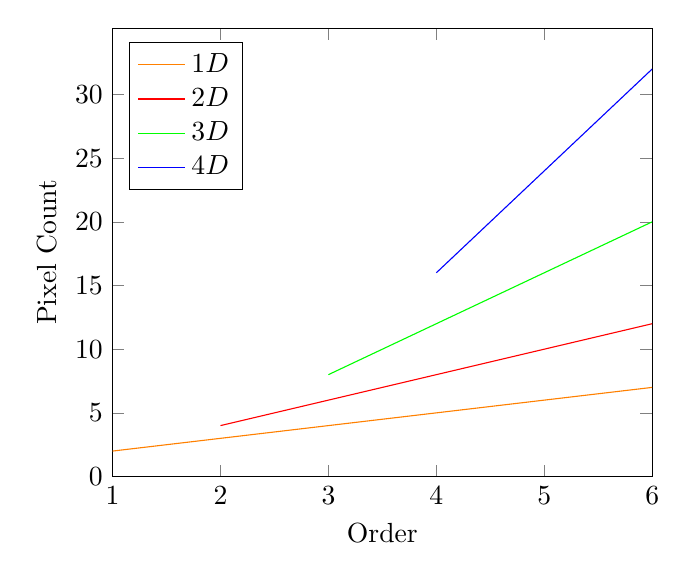
\begin{tikzpicture}

      \begin{axis}[xmin=1,xmax=6,ymin=0,xtick={1,...,6},ytick={0,5,10,15,20,25,30},xlabel={Order},ylabel={Pixel Count},legend pos=north west]

        % 1d textures
        \addplot[color=orange, domain=1:6]{x+1};
        \addlegendentry{$1D$}

        % 2d textures
        \addplot[color=red, domain=2:6]{x*2};
        \addlegendentry{$2D$}
    
        % 3d textures
        \addplot[color=green, domain=3:6]{(x-1)*4};
        \addlegendentry{$3D$}

        % 4d textures
        \addplot[color=blue, domain=4:6]{(x-2)*8};
        \addlegendentry{$4D$}        
            
      \end{axis}
    \end{tikzpicture}

    \caption{Pixel count for curve order, with different texture dimensionalities.}
    \label{fig:pixelcount}
  \end{figure}

%-------------------------------------------------------------------------
\section{Extensions}
\label{sec:extensions}

There are a few ways to extend this technique for more options.

\subsection{Combining Color Channels}

If you encode Bezier curves into a texture which has multiple color channels - such as the standard four R,G,B,A - you can set up the textures such that once you read in the R,G,B,A, you can combine the channel values together such that you get a fewer number of curves per texture read, but that they are higher order.

For instance, if you had a 2x2 texture, you could encode the control points A,B,C into the red channel, and the control points B,C,D into the green channel.  Then, after you did a texture read, you could do a lerp between the red and the green channel.  Since the red and green channel each contain a quadratic curve, the result would be a cubic curve, defined by the control points A,B,C,D.  However, you've used up two of the channels for a single curve, so are getting fewer curves per texture read, but they are higher order.  The blue and the alpha channel could either be quadratic curves, or could also be encoded such that they could be combined together to provide another cubic curve.

You could also set it up such that R,G,B,A were meant to be combined together to make a quintic (degree 5) curve.  You'd only get a single curve value per texture read, but it would be 3 degrees higher.  You could combine the color channels either with De Casteljeau's algorithm, or with the cubic Bernstein Bezier form. 

If you you are combining M color channels, each of which are values from curves of order N, the resulting curve value will be order N+M-1.  The intuitive explanation to this, is that each channel has the ability to add one more control point to the curve, regardless of what texture dimensionality you are working with.

An interesting side effect to combining color channels is that the accuracy of the resulting curve gets better.  This is because you are doing some of the math in full precision floating point, instead of the limited precision of the fixed point math in the texture sampler.

\subsection{Piecewise Curves}

As mentioned earlier, you can encode multiple Bezier curves end to end within textures of any dimensionality.

When you are in need of a curve with lots of control points, piecewise curves have several benefits over increasing the order of the curve.

The main benefit of piecewise curves are that they allow us to use lower order curves, which allows us to use lower dimensional textures, and have less computation in the shader programs.

Another benefit is that there can be discontinuities between curve segments, which is sometimes desired by artists and graphic designers.

B-splines can also be converted to piecewise Bezier curves using Boehm's algorithm, so even though this technique only explicitly deals with Bezier curves, B-splines could be converted to piecewise Bezier curves and could be used in that form.

Evaluating a piecewise curve with this technique is very simple.  As an example, let's say that we have a texture that is 8x2, and encodes 4 quadratic Bezier curves end to end. The left most 2x2 pixels encode the quadratic curve used for time $t \epsilon [0,0.25)$.  The next block of 2x2 pixels encode the quadratic curve used for time $t \epsilon [0.25,0.5)$.  The third block encodes time $t \epsilon [0.5,0.75)$, and the last block encodes time $t \epsilon [0.75,1.0]$.

\subsection{Rational Bezier Curves}

\begin{figure}
    \begin{tikzpicture}[x=12cm,y=6cm]
      \node[anchor=south west,inner sep=0] at (0cm,0cm) {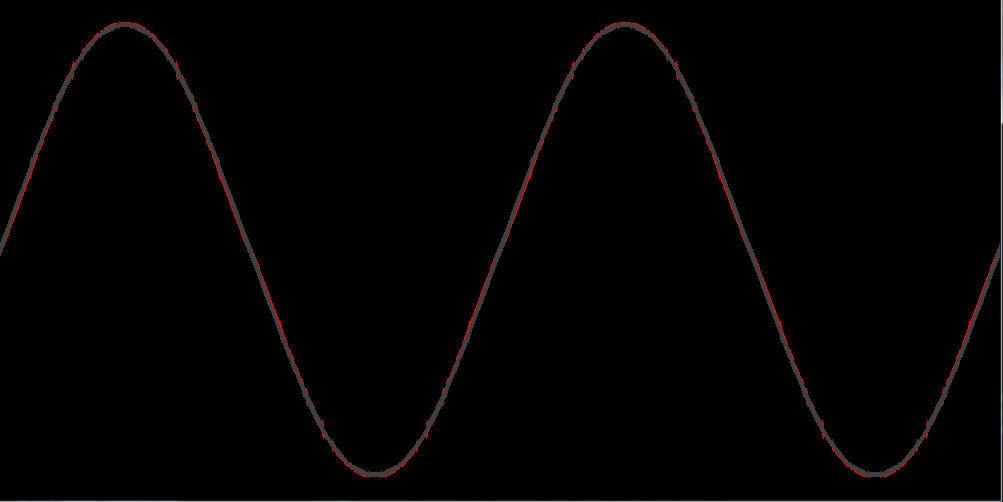
\includegraphics[width=12cm,height=6cm]{Rational.png}};  
    \end{tikzpicture}

    \caption{A rational bezier spline showing cosine in green and sine in red.  The white line is the true value of those functions. \textit{Left:} Evaluated with hardware sampling and then division.  \textit{Right:} Evaluated by reading the control points into the shader program, calculating the curves, and then doing a division.}
    \label{fig:rationalbeziersincos}
  \end{figure}

Rational Bezier curves are useful because they can be used to make shapes which cannot be formed from integral Bezier curves, including perfectly representing conic sections.  This also means that they can accurately represent sine and cosine as seen in \autoref{fig:rationalbeziersincos}.  Rational Bezier curves are defined by the equation:

\begin{equation}
\text{\bf{B}}(t) = \frac
                % Nominator
                {\sum\limits_{i=0}^n\binom {n} {i}(1-t)^{n-i}t^iw_i\text{\bf{P}}_i}
                % Denominator
                {\sum\limits_{i=0}^n\binom {n} {i}(1-t)^{n-i}t^iw_i}
\label{eqn:rationalbezier}                
\end{equation}

If we were to multiply the weight into the control point for the numerator, We can see that we essentially have one Bezier curve divided by another.  Using the techniques in this paper, we could easily encode the numerator into one color channel, and the denominator into another.

If we wanted to get two rational Bezier curves per texture read, we could encode the two numerators into R and G, and the denominators into B and A.

Or, if we had three curves that all used the same weights, that would mean that the denominator was the same for all three curves.  In this case, we could encode the three numerators into R,G,B and encode the denominator in A, which would give us three rational curves with a single texture read.

To compute the value of rational Bezier curves, you first take your texture samples, combining them as per normal if there were multiple taken (if needed), and then after that, you divide the numerators by the denominators to get the final values.

There is a limitation to encoding rational Bezier curves in this form due to the fact that texture values range from 0 to 1, but when using rational Bezier curves, weights greater than 1 are sometimes desired.  The good news is that you can normalize the weights by dividing all weight values by the largest weight value, such that the largest weight value becomes 1.  The result will be the same as if you had values greater than 1 in the weights.

Just as b-splines can be converted into piecewise Bezier curves, NURBS can also be converted into piecewise rational Bezier curves, again using Boehm's algorithm, which means these techniques can also apply to NURBS, if they are first preprocessed into rational Bezier curves.

\subsection{Multidimensional Bezier Curves}

So far we have only talked about one dimensional --- or explicit --- Bezier curves which take the form of $y=f(x)$.  Multidimensional Bezier curves are evaluated separately per axis though, which means that you can encode information per axis in different color channels.

To name a few possibilities with a standard RGBA 2x2 texture, you could encode a fourth dimensional Bezier curve, or you could encode 2 two dimensional Bezier curves, or you could even encode a three dimensional rational Bezier curve using R,G,B for the numerator of each axis, and A as the denominator for all three curves.

%-------------------------------------------------------------------------
\section{Addressing Accuracy Issues}
\label{sec:addressingaccuracyissues}

  \begin{figure}
    \begin{tikzpicture}[x=12cm,y=4cm]
      % border
      \draw (0cm,0cm) rectangle (12cm,4cm);
      % images
      \node[anchor=south west,inner sep=0] at (0cm,0cm) {
\includegraphics[width=4cm,height=4cm]{SampleHW.png}};
      \node[anchor=south west,inner sep=0] at (4cm,0cm) {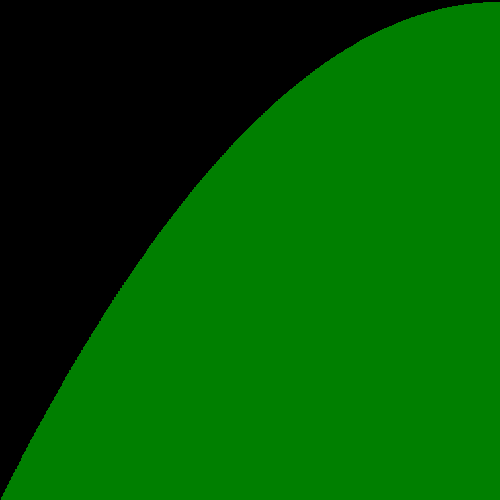
\includegraphics[width=4cm,height=4cm]{SampleHWSW.png}};
      \node[anchor=south west,inner sep=0] at (8cm,0cm) {
\includegraphics[width=4cm,height=4cm]{SampleSW.png}};   
          
    \end{tikzpicture}
    \caption{\textit{Left:} Curve evaluted with a single texture read and bilinear texture sampling.  \textit{Middle:} Curve evaluated with two linear texture samples, combined in the shader program.  \textit{Right:} Curve evaluated with three texture samples (one per control point), combined in the shader program.}   
    \label{fig:samplehwsw}
  \end{figure} 

Even though there are accuracy limitations in modern GPU texture samplers, accuracy can be increased by doing more of the calculations in the shader program, which operate at full floating point precision.

A naive way to do this would be to use nearest neighbor texture sampling instead of linear, and do the linear interpolations yourself in the shader program.  This would mean twice as many texture reads with a 1D texture, four times as many texture reads with a 2D texture, and eight times as many texture reads with a 3D texture.  You would also be doing a lot more blending in the shader program, so your shader programs would become heavier weight.  This solution is essentially doing software linear texture sampling.

A better approach that gives the same results would be to only do one nearest neighbor texture sample per control point in the texture, and then in the shader program, either use De Casteljeau's algorithm to combine them, or use the Bernstein form equation of Bezier curves.  At this point, you are best off just using a 1D texture to store your control points in, since you don't need any of the built in interpolation.

These two techniques do all of the curve math in the shader program at full floating point precision and so are the highest quality, but are also the most computationally expensive.

Another way to address accuracy would be to do some of the work in the texture sampler, and some of the work in the shader program.  This allows you to have a sliding scale for accuracy vs cost.

For instance, if you had a 2x2 image which encoded a quadratic Bezier curve, you might do two texture reads, letting the texture sampler do the $x$ axis interpolation, and then you could linearly interpolate those results in the shader program in full precision floating point math for the $y$ axis.  This would give you a result somewhere between full hardware and full software interpolation.  You can compare the results in \autoref{fig:samplehwsw}.

Also, if you want a higher order curve than your texture can provide with a single read, forcing you to combine multiple curve points, combining those curve points in the shader program has the nice side benefit of increasing accuracy as well.

%-------------------------------------------------------------------------
\section{Limited Applications for Vector Graphics}
\label{sec:limitedapplicationsforvectorgraphics}

This technique does have applications to vector graphics, but they are pretty limited and there are better solutions if using Bezier curves as vector art is the goal \cite{Loop:2005:RIC:1073204.1073303,Nehab:2008:RRG:1409060.1409088}, or if the goal is to use textures for vector art data storage \cite{Green:2007:IAM:1281500.1281665}.  The limitation is due to the fact that this technique is good at calculating the point on a curve at time $t$, but when using curves in vector graphics situations, you usually do not know the time $t$ that you want to know the curve point for, and it is usually difficult to find it.

However, there are certain special situations where you can easily get the time $t$ value of the curve that you care about.  Two of the most common situations for these are when rendering 1D explicit Bezier curves, and when rendering 1D explicit Bezier curves in polar form.

Explicit Bezier curves are curves which have scalar control points and are in the form of $y=f(x)$.  For these curves, when you plug in a value for $x$ you get a $y$ value out.  They are unable to make curves that have multiple $y$ values for the same $x$, and the curves can't cross over themselves to make closed shapes.  This does make them not as useful to vector graphics as 2D Bezier curves which are of the form $(x,y) = f(t)$, but they still do have some use cases.  Rendering explicit Bezier curves using this technique is very simple.  If rendering a quad, you just choose either the $x$ or $y$ axis, normalize it from 0 to 1 and use that to calculate the other axis value by doing a texture sample.  At this point, you can either choose a half space to color in, or you can calculate the gradient of the function (by using the built in dFdx style functions to get partial derivatives), and use that as an estimated distance to the curve.

This idea can easily be extended to 1D Bezier curves rendered in polar form.  If rendering a quad, you can use arc tangent to find the angle of the current pixel from the center, normalize that angle to 0 to 1, and then use that value to do a texture look up to calculate the value of the curve at that point.  Once again you can then either choose a half space to color in, or you can use the gradient information to get an estimated distance to the curve, to draw a curved line.

Another problem with using this technique for vector graphics, is that since the texture sampler is doing at least some of the calculations for us, we don't have access to the values of the control points, which can make some operations harder.  Luckily, one property of Bezier curves is that affine transformations done to control points is equivalent to affine transformations done to points on the curve.  This means that we can do affine transformations on the curve points provided to us by the texture sampler, and it will be as if we had performed them on the control points themselves.

Lastly, in regards to vector graphics, this technique can be used to allow people to define custom color gradients.  The benefit is that custom, non linear color gradients can be defined, and can be zoomed into without decaying to linear interpolation.

  \begin{figure}
    \hspace{-1.5cm}
    \begin{tikzpicture}[x=16cm,y=4cm]
      % images
      \node[anchor=south west,inner sep=0] at (0cm,0cm) {
\includegraphics[width=8cm,height=4cm]{Flag.png}};
      \node[anchor=south west,inner sep=0] at (8cm,0cm) {
\includegraphics[width=8cm,height=4cm]{FlagZoom.png}};
    \end{tikzpicture}
    \caption{\textit{Left:}An animated flag textured with vector graphics using the techniques in this paper, using an 8x4 RGBA source texture to generate curves and color gradients.  \textit{Right:} Zooming in on part of the image to show the quality of the vector graphics.}   
    \label{fig:vectorgfx}
  \end{figure}

A demonstration of these usage cases can be seen in \autoref{fig:vectorgfx}.

%-------------------------------------------------------------------------
\section{Performance Characteristics}
\label{sec:performancecharacteristics}

The table below was created by running a 1000x1000 pixel shader program where each pixel evaluated a curve using either linear texture sampling (HW or hardware evaluation), or did multiple texture reads to get the control points and then calculated the curve values inside of the shader program (SW or software shader program evaluation).  The numbers shown are the time spent rendering each frame, in microseconds and the texture format is R8G8B8A8.  Actual performance characteristics in real world scenarios will be based on other factors, such as whether the texture is in the texture cache, or whether you are texture fetch bound or compute bound in the shader program.

\begin{tabular}{|l|l l|}
\hline
& \multicolumn{2}{|c|}{NV GF GTX 980m} \\
& \bf{HW} & \bf{SW}\\ \hline
\bf{1D Texture / Linear Curve} & 131.8 $\mu$s & 132.7 $\mu$s \\ \hline
\bf{2D Texture / Quadratic Curve} & 131.1 $\mu$s & 135.1 $\mu$s \\ \hline
\bf{3D Texture / Cubic Curve} & 135.4 $\mu$s & 146.2 $\mu$s \\ \hline
\end{tabular}

TODO: do a test with the cards at work, and put those results here as well!

%-------------------------------------------------------------------------
\section*{Future Work}
\label{sec:futurework}

In the past, work has been done to evaluate curves on the GPU using textures, but for the purposes of texture interpolation \cite{doi:10.1080/2151237X.2008.10129269}.  The progress made on those types of techniques could likely be used in a similar fashion to directly evaluate other curve types on the GPU for purposes other than texture sampling.

Extending this technique to the third dimension would be an interesting usage case, as well as exploring ways to make the vector art usage cases more attractive.

There may also be usefulness in curves in polar form to approximate lobes for lighting algorithms.

Lastly, throughout this paper, texture coordinates were set up such that the texture samples were taken only across the diagonal of $N$-dimensional hypercubes.  It would be interesting to explore whether deviating from the diagonal created useful properties, more complex curves, or more complex curve types so that even more usefulness could be achieved with the same number of pixels used.

%-------------------------------------------------------------------------
\section*{Acknowledgements}
\label{sec:acknowledgements}
TODO: this


%-------------------------------------------------------------------------
\small
\bibliographystyle{jcgt}
\bibliography{paper}

%-------------------------------------------------------------------------
\section*{Index of Supplemental Materials}
\label{sec:indexofsupplementalmaterials}
TODO: this


%-------------------------------------------------------------------------
\section*{Author Contact Information}

\hspace{-2mm}\begin{tabular}{p{0.5\textwidth}p{0.5\textwidth}}
Alan Wolfe \newline
Blizzard Entertainment \newline
16215 Alton Parkway \newline
Irvine, CA 92618 \newline
\href{mailto:awolfe@blizzard.com}{awolfe@blizzard.com}
\href{http://blog.demofox.org}{http://blog.demofox.org}
\end{tabular}


\afterdoc

\end{document}
